\documentclass{article}\usepackage[]{graphicx}\usepackage[]{color}

\usepackage{alltt}
\usepackage{float}
\usepackage{graphicx}
\usepackage{tabularx}
\usepackage{siunitx}
\usepackage{amssymb} % for math symbols
\usepackage{amsmath} % for aligning equations
\usepackage{textcomp}
\usepackage{booktabs}
\usepackage{mdframed}
\usepackage{natbib}
\usepackage{comment}
\usepackage{booktabs}
\usepackage[colorinlistoftodos]{todonotes} % to make comments on the margin
\usepackage[small]{caption}
\setlength{\captionmargin}{30pt}
\setlength{\abovecaptionskip}{0pt}
\setlength{\belowcaptionskip}{10pt}
\topmargin -1.5cm        
\oddsidemargin -0.04cm   
\evensidemargin -0.04cm
\textwidth 16.59cm
\textheight 21.94cm 
%\pagestyle{empty} %comment if want page numbers
\parskip 7.2pt
\renewcommand{\baselinestretch}{1.5}
\parindent 0pt
%\usepackage{lineno}
%\linenumbers

%% R Script

\title{Unravelling the phenology-phylogeny tangle.}

% alternative titles:
%% An expanded bayesian phylogenetic mixed model to unravel the phenology-phylogeny tangle. %% this sounds too methodsy

\begin{document}

\maketitle

\noindent Authors:\\
The Wolkovich Lab in 2019 \& collaborators $^{1,2,3,4}$ % Will Pearse, Jonathan Davies also
\vspace{2ex}\\
\emph{Author affiliations:}\\
$^{1}$Forest \& Conservation Sciences, Faculty of Forestry, University of British Columbia, 2424 Main Mall, Vancouver, BC V6T 1Z4;\\
$^{2}$Arnold Arboretum of Harvard University, 1300 Centre Street, Boston, Massachusetts, USA;\\
$^{3}$Organismic \& Evolutionary Biology, Harvard University, 26 Oxford Street, Cambridge, Massachusetts, USA;\\
$^{4}$Edificio Ciencias, Campus Universitario 28805 Alcalá de Henares, Madrid, Spain\\
 

\vspace{2ex}
$^*$Corresponding author: ignacio.moralesc@uah.es\\
\renewcommand{\thetable}{\arabic{table}}
\renewcommand{\thefigure}{\arabic{figure}}
\renewcommand{\labelitemi}{$-$}
\setkeys{Gin}{width=0.8\textwidth}

%%%%%%%%%%%%%%%%%%%%%%%%%%%%%%%%%%%%%%%%%%%%%%%
%%%%%%%%%%%%%%%%%%%%%%%%%%%%%%%%%%%%%%%%%%%%%%%
\clearpage



%%%%%%%%%%%%%%%%%%%%%%%%%%%%%%%
% Results & Discussion
%%%%%%%%%%%%%%%%%%%%%%%%%%%%%%%

%%%%%%%%%%%%%%%%%%%%%%%%%%%%%%%
% Discussion
%%%%%%%%%%%%%%%%%%%%%%%%%%%%%%%

%\section*{Discussion}
% EMW (26Apr2022): Some great text here! Would flow really well with a combined R&D.
%IMC 06may - Giving a try at merging Results and Discussion below


\section*{Results \& Discussion}
% Are we in past or present tense here? (asks Lizzie)

Most species are sensitive to all three primary cues---forcing, chilling, and photoperiod (Figs. \ref{fig:muplot_all}, Supporting Table \ref{tab:})\citep[see also][]{Laube:2014a,ettinger2020}---with sensitivity to chilling approximately five-fold greater than sensitivity to photoperiod, on average (phenological advances of 7.2 days per standardized unit vs 1.4 days, for chilling and photoperiod, respectively; see Table \ref{tab:modelanglamb}). However, these average sensitivities estimated across species, fail to capture the large differences in responses to chilling and forcing among species (Figs. \ref{fig:muplot_all}, Supporting Table \ref{tab:}). 

By allowing species responses to vary, using a model that explicitly accounted for species' shared evolutionary history, we found species differences dwarfed the magnitude of differences between cues (Fig. \ref{fig:muplot_all}): chilling varied 25-fold between species, while variation to forcing varied 6-fold. Our results suggest the strong focus on comparing cues misses the largest source of variation in phenological responses. Robust phenological forecasts must account for both the complexity of multiple cues and species-level variation in responses to them.

\emph{Differences across clades \& cues}

The large differences across species, however, were not random, but showed strong phylogenetic patterning, producing striking differences between clades. For example, oaks and beeches (Fagaceae), elms (Ulmaceae) and buckthorns (Rhamnaceae) are highly sensitive to chilling while rhododendrons (Ericaceae), butterfly bushes (Scrophulariaceae) or spindles (Celastraceae) show little to no response to chilling (Fig. \ref{fig:muplot_all} a). %IMC: not sure if we need some natural history here or some mention to research for some of these clades. Lizzie, if you want to mention-cite something here, please jump in. % EMW (21Nov2022 and 1 Dec2022) I can work with JD to add more here later.
% JD I think some biogeography may be useful here, for example, I think rhododendrons & buddleia are native to the Himalaya, but both are also now widespread and invasive ... need to do a little more digging on the exact species.   
Similar clade-level variation was observed for forcing, where some clades---e.g., Ericaceae, Rhamnaceae, Ulmaceae, and Fagaceae---were particularly sensitive (advancing their budburst more than 10 days per standardized unit of forcing), while  others such as the Sapindaceae, Cornaceae or Juglandaceae families showed only weak response (Fig. \ref{fig:muplot_all} b). %JD - perhaps could link back to invasiveness? Species more sensitive to forcing more invasive?

In the data analysed, we found that some species responded strongly to both temperature cues (chilling and forcing), which could suggest the existence of syndromes where the genetic basis for responses to one cue (e.g., forcing) has been been selected for alongside responses to another cue (e.g. chilling). We might expect, for example, early-season species to be sensitive to multiple cues as mistiming phenology could result in exposure to harsh conditions, leading to tissue loss or death \citep{frostbook}, and sensitivity to multiple cues likely provides greater insurance against mistiming \citep{memegan2021}. Alternatively or additionally, linkage or pleiotropism among loci associated with sensitivity to different cues \citep{nakagawa2005} could induce correlated cues. However, the correlation in species sensitivities across cues was weak (\emph{r} = 0.31; between forcing an chilling) and some genera, such as \emph{Tilia} and Ericaceae[genus?], displayed strong responses to forcing but weak responses to chilling, while others, such as XXXXExamplesXXXX, show strong responses to chilling but weak responses to forcing (Fig. \ref{fig:muplot_all}). Species sensitivity to one cue, thus, does not constrain sensitivity to another cue, and selection might operate independently on responses to different cues \citep{bonamour2019}.

In contrast to both chilling and forcing, species-level responses to photoperiod were of smaller effect and almost uniform across species. This observation provides novel insight on a large debate over the prevalence of photoperiod cues in temperate trees, where previous experiments  \citep{Basler:2012,zohner2016} and modeling exercises \citep[e.g.,][]{Hunter:1992jw,schaber20203} indicated important variability across species that could constrain the responses of certain species to warming \citep{way2015}. Our results suggest variability is broadly limited to a handful of species in Fagaceae, which have been heavily studied, such as \emph{Fagus sylvatica} \citep[e.g.,][]{Basler:2012,zohner2016,kramer2017}. Perhaps not coincidentally, these same few species are also where we find most evidence of local adaptation in photoperiod cues \citep[e.g.,][]{kramer2017}. Given that studies included in our analysis spanned a range of latitudes (with many species studied in only a narrow latitudinal range), if local adaptation was high in photoperiod cues we would have expected more variability across species. The uniformity of response to photoperiod that we found thus supports an alternative view of generally low local adaptation in photoperiod cues for spring phenology, consistent with common garden studies of other species, which have reported little evidence of local adaptation in spring (but not fall) phenology \citep{aitken2016}.

Our results suggest that while chilling and forcing are the dominant cues in terms of the magnitude of their effect sizes, most species are also sensitive to photoperiod, highlighting the potential importance of this cue to both climate change responses in the future, and through evolutionary history. In plants, photoperiod regulates a number of fundamental processes including growth, flowering, stress tolerance, and circadian rhythm \citep{serrano2017,Singh:2017}, with photoperiodic sensing and adaptation to shifting daylength likely occurring early in the evolution of plants, perhaps with origins in the green algae \citep{serrano2017}. It is possible, therefore, that phenological responses to photoperiod reflect ancestral sensitivities with origins in deep time. Large plasticity in responses to additional environmental cues (e.g., temperature) for a given photoperiod cue \citep[e.g.,][]{kramer1995} may allow species to track interannual variation in climate with little directional selection on photoperiod sensitivities. Alternatively, photoperiod might provide a reliable calibration of the underlying biological clock \citep{jackson2009plant} upon which seasonal variation in climate modifies the tempo. 
%JD - I still need to get to grips with what is going on with photoperiod, low lambda is consistent with rapid evolution within species, but low sigma suggests low rates of evolution. Perhaps photoperiod is dominated by local adaptation, but little directional selection, so local adaptation just gets washed out overtime?

\emph{Phylogenetic structure of phenological cues}

Variation---or lack thereof---in cues across species and clades, alongside related parameter estimates from our phylogenetic modeling approach, provides unique insights into the evolution of cues across the plant tree of life. While responses to each cue were phylogenetically structured, the strength of phylogenetic conservatism in responses differ between cues (Fig. \ref{fig:phylosig_all}). Responses to temperature (forcing and chilling) were moderately structured ($\lambda = 0.65$ and $\lambda = 0.54$, for forcing and chilling, respectively), such that closely related species exhibiting more similar sensitivities than distantly related species. However, phylogenetic structure in species responses to photoperiod was comparatively weaker ($\lambda= 0.39$) (see Fig. \ref{Fig:muplot_all}, Table \ref{tab:modelanglamb}), emphasizing again that photoperiod diverges from other climate cues. In addition to being weaker and more uniform across species, sensitivity to photoperiod appears to also be less evolutionarily constrained than sensitivities to temperature cues. % While our approach is unique in focusing on species cues, our results support previous work showing phylogenetic signal in plant phenological timing observed from floras or long-term data \cite{kochmer1986constraints,davies2013phylogenetic}. 

What might drive phylogenetic structure in species temperature responses? Differences between species in their responses represent shifts in the slope of the relationship between the observed phenology and the cue. Thus, the observed phylogenetic structure in temperature responses (forcing and chilling) would be consistent with an interaction with a non-measured trait that moderates responses, and which also covaries with phylogeny \citep{davies2019phylogenetically}. This fits fundamentally with the idea that early-season phenology plays a critical role in shaping species temporal niches \citep{gotelli1996} and thus should covary with a suite of life-history traits, including whether species are early-active with rapid return on investment trait, or start later in the season and have traits associated with higher competitive abilities \citep[e.g.,][]{Grime:1977sw,wolkovich2014aob}. Geography may additionally drive structured phylogenetic variation, especially in regions where clades have radiated such that close relatives have experienced the same suite of environmental cues and thus been subject to similar selection regimes over their evolutionary history. Conversely, if species are not generally geographically constrained, as may be more likely the case, especially across deep time \citep{fitzturelli2006}, then we might expect phylogenetic structure in phenology to also weaken, especially when aggregating across locations with different cues \citep{davies2013phylogenetic}.%JD: could cut last sentence

% EMW (21Nov2022): Do we want to mention any molecular work on photoperiod (or other cues)?
Weak phylogenetic signal in photoperiod sensitivity (Fig. \ref{fig:phylosig_all}) might seem at odds with observations that distantly related species respond more similarly (and less variably) to photoperiod than they do to forcing or chilling. However, somewhat counterintuitively, both uniform and random responses can manifest as low phylogenetic signal when estimated relative to Brownian motion expectations (see Wiens et al.). For example, rapid local adaptation within species might erase the phylogenetic structure in photoperiod responses, but this scenario is inconsistent with the uniformity we find in species' responses. Alternatively, if responses to photoperiod evolved early in plants, as we suggest above, and subsequent selection on photoperiod sensitivity was constrained by stabilizing selection operating on other life-history attributes sensitive to photoperiod \citep[e.g.,][]{Rinne:1994,Wilczek2014,azeez2015}, we would predict both low interspecific variation and weak phylogenetic signal in responses, better matching our observations. This latter interpretation is also consistent with our estimates of lower $\sigma$ for photoperiod responses (CITE FIGURE). Here, as in more traditional phylogenetic comparative methods, $\sigma$ represents the rate of evolution, and thus our results suggest photoperiod responses are also evolving slower than temperature responses. As we also show (see Appendix XXX), lower $\sigma$ may capture the evolutionary dynamics of an 'early burst' model, in which trait variation accumulates rapidly early in the history of a clade and then slows through time (XXXcite Harmon: https://doi.org/10.1111/j.1558-5646.2010.01025.x), concordant with our interpretation of photoperiod evolution.
%JD - Call out to Will for assistance ...

Phylogenetic conservatism (high $\lambda$) and slow evolutionary rates (low $\sigma$) in traits has sometimes been interpreted as indicative of evolutionary constraints to adaptive change (cite Wiens et al. and others cites XXX). If this were the case, we might then suggest that species with strong forcing response might be more vulnerable to future warming because phylogenetic conservatism ($\lambda$) in responses to forcing is higher compared to other cues, and its evolutionary rate ($\sigma$) is lower. This is misleading, however, as estimates of $\lambda$ are independent from the rate of evolution, and macroevolutionary rates estimated on phylogenetic trees that integrate across millions of years of evolutionary history, and thus do not necessarily inform us of maximum possible rates of evolution over much shorter timescales. Indeed, there is accumulating evidence for rapid evolution to shifting climates \citep{bradshaw2006,franks2014}. Our estimates of phylogenetic structure are thus more useful in improving our understanding of the evolutionary history of species phenological cues and how they should be modelled, and emphasise the importance of robustly estimating species differences in ecological forecasts. %JD - Call out to Will for logic-checking ...

% I'm commenting out this bit but leave it here in case we want to mention some of it in methods or an appendix
%From a statistical perspective, accounting for the effects of phylogenetic structuring on the effects of jointly modelled cues had an effect on model coefficients (Fig. \ref{fig:correls_angio}). Not accounting for phylogeny (or assuming $\lambda$ = 0) biased model coefficients, particularly so for forcing and somewhat less for chilling (Fig. \ref{fig:correls_angio}). Specifically, species sensitivities to forcing and chilling were underestimated on average (model slopes shifted by 7.2\% and 3.7\%, respectively). Sensitivities to photoperiod, which showed weak phylogenetic signal were not biased in non-phylogenetic models (Fig. \ref{fig:correls_angio}), likely associated to their low estimated $\lambda$ values. Model intercepts were not affected either (Fig. \ref{fig:correls_angio}).\\ 

\emph{Forecasting species-level responses}

Our results highlight that species-level variability can be extremely high---when properly estimated. Our approach, which partially pools species responses based on their shared evolutionary history, did not have large influence on the average coefficients across species (model slopes for forcing and chilling shifted by 7.2\% and 3.7\%, respectively; Fig. \ref{fig:correls_angio}), but estimated substantially higher variation among species compared with widely used hierarchical models. This was especially noticeable in temperature responses (for chilling variance across species was $\beta_{phylo}$ = 23.45 compared to $\beta_{non-phylo}$ = 17.47, for forcing it was $\beta_{phylo}$ = 8.74 compared to $\beta_{non-phylo}$ = 5.01) while photoperiod, which had low phylogenetic structure was more similar across approaches (variance of $\beta_{phylo}$ = 0.82 compared to $\beta_{non-phylo}$ = 0.93). Counterintuitively, a reduction in cross-species variance, far from increasing model accuracy could lead to increased type-II error by failing to detect actual relationships among cues and responses that would only emerge when phylogeny is correctly accounted for (see Supporting Information XX). % EMWDec1 -- I am not sure what we mean in this last sentence, but it sounds important ... but since I am not sure what we mean I apologize if I put it in the wrong place 
%JD I have tinkered with this a little, not sure it is an improvement

%JD: merge following two sentences with paragraph above?
Importantly, the increase in variability across species allowed for in our model with phylogenetic structure decreased the uncertainty in estimates for individual species' temperature responses. Thus, traditional approaches that partially pool across species ignoring ther evolutionary affiliations (i.e. most hierarchical models in ecology) may lead to less precise predictions for individual species, although overall model accuracy might still appear reasonable (see Appendix XX in Supporting Information).%JD: not sure what is meant by overall model estimates/accuracy, I assume this is the mean slope or some such ...

% EMWDec1 -- need to check below about oaks and make sure we see this difference in lamba0 models... (and we could perhaps contrast this oak bit a little more)
Our model help inform which clades will be more sensitive to different axes of climate change---e.g., changes temperatures over winter (associated with chilling) versus spring (associated with forcing). For example, using a hierarchical model would not have identified oaks (genus \emph{Quercus}) as being among the most sensitive to forcing and chilling (see e.g., \citep{ettinger2020}), but we show that species within this genus advance phenology by 2 days per standard unit of forcing and 4 days per standard unit of chilling. Our analyses highlight the need to move beyond current very general classifications currently used in models \citep[e.g., functional groups ... Cat/Dan, can you offer better ref?][]{Moorcroft:2003dz} or groupings at coarse taxonomic levels \citep[e.g.,][]{ettinger2020} to make improved ecological forecasts for individual species. 

The contrasts between temperature sensitivities and photoperiod sensitivities---in both their variability across species and phylogenetic structure---also allow for improved multi-species forecasts. For temperature responses, the large variability among species makes predicting species' individual responses challenging, but the phylogenetic structure in responses lets us borrow  information from close relatives to improve our estimates. While this must be done with care \citep{molina2018assessing}, especially given our very limited sampling of species, our results could provide reasonable predictions for many temperate woody plant species from clades for which we have multiple species and experimental observations at varying treatment levels. For photoperiod, the weak phylogenetic structure in responses indicate that phylogeny retains little information, but because species responses are generally more uniform, we can be more confident in assuming the mean species response across species, comforted in the knowledge that small errors will likely not have large impact given the relatively weak overall contribution of this cue, except for \emph{Fagus sylvatica}. As \emph{Fagus sylvatica} is nearly five times more sensitive to photoperiod than most other measured tree species, our results caution against using it to draw inferences of photoperiod responses more widely. 
% The genus \emph{Fagus} is recognized as being particularly sensitive to photoperiod \citep{fu2019}. Specifically, \emph{Fagus sylvatica} is nearly five times more sensitive to photoperiod than most other measured tree species. The question arises as to whether species with outlying responses should be chosen as the model from which to extrapolate knowledge as done with \emph{Fagus sylvatica} in the phenology literature (REFs for PEP75?!). %HELP with references on Fagus would be appreciated. % EMW (21Nov2022) I'll add more here later

While we focused on spring phenology here, our modeling approach suggests a path towards more robust forecasting via integrating species-level estimates of climate change responses. Our results show how including the phylogenetic relationships among species can overcome major limitations of most current hierarchical models (producing biased model estimates, underestimating the full variability across species, and increasing uncertainty around individual species' estimates) while at once providing insight into the evolutionary history of biological responses. [And, bam, something a little more here ... ]
%JD: could give a nod to how our model might also be applied to forecasting geographical/range shift responses etc. However major challenges remain, for example, obtaining data across representative species to fit models, and then scaling up model predictions at the species level to ecosystems (weather -> climate!).  

%IMC- I'm commenting out this paragraph as I'm not sure we want to discuss intercepts. in 20nov meeting we decided not to talk about this unless Will feels we should and has something to add to this paragraph.
%Our models found non-negligible phylogenetic signal in model intercepts (see \ref{fig:phylosig_all}). This indicates that the intrinsic variation across species in the timing of budbreak before experiencing the effects of any environmental cue, is also phylogenetically patterned. This is, regardless the action of cues some tree species budbreak earlier than others, and these differences tend to be smaller, at least to some extent (the signal is weak $\lambda$ = 0.35), among closely related species. Previous work had already shown large variation across species in their model intercepts \citep{davies2013phylogenetic}. % not sure this is the right citation, ask Lizzie. This whole paragraph needs work (based on conversation over coffee May6th).  While fitted species-level intercepts did not change between the phylogenetic and non-phylogenetic model (\ref{fig:correls_angio}), our approach suggests that the mechanisms underlying species' baseline phenological differences would not operate randomly across the phylogeny.\\    

% EMWDec1 -- commenting out the below, it has some good stuff we could later tuck into the abstract or this section (especially the second chunk -- which I have deleted here and moved to abstract), but feels repetitive to me mostly given the current text. 
% Accurate forecasts of phenology remain elusive; recent records have suggested an apparent decline in species phenological sensitivity to increasing temperatures \citep{fu2015,piao2017}, but such observations may simply reflect non-linear responses to warming trends \citep{wolkovich2021simple}, perhaps reflecting the complex interactions, trade-offs and synergies among multiple cues. While all species appear sensitive to all cues, forcing and chilling dominating over photoperiod, and species-level variation in responses is large, of a magnitude similar to, or greater than, the difference in average effect sizes between cues. Phylogenetic conservatism in species phenology has been well documented \citep{davies2013phylogenetic,rafferty2017global,joly2019importance}, and may thus help explain species differences. 

%\subsection*{Model accuracy}
%IMCapr25 - I'd like to include a little subsection here on model accuracy, comparing R2s, LOO, or something similar for our models. Unfortunately, I can't find an easy way to do that (for stanfit objects: https://discourse.mc-stan.org/t/best-way-to-do-prediction-on-new-data-r-rstan-stanfit/1772/17) any help with this is much appreciated. 
% EMW (26Apr2022): To use loo we just need a generated quantities block, right? If so I can try to help code that with Deirdre.
%IMCmay10- I re-run models storing yhats as a generated quantity, and with that computed a Bayes version of R2. There's not change in accuracy between our approach and the lambda0 approach, but accuracy drops if lambda is forced to be equal1. 

%angio
%R2lamb0 0.666
%R2lambest 0.665
%R2lamb1 0.657

%gymno
%R2lamb0 0.527
%R2lambest 0.530
%R2lamb1 0.498

%\item How can we interpret lambdas and sigmas for each cue, and for the intercept?
%\item What are the implications for phenological predictions and forecasts?
%\item Is this approach transferable to different taxa or biological responses? 
%\item Do results differ from what would be expected if single cues where analyzed separately, phylo or non-phylogenetically?


%\item If so, can accounting for phylogeny shed light on the ongoing debate on declining sensitivities? For example, if particular lineages have very different evolutionary constraints on their responses to the cues, they may also display very differt declines in their sensitivities to the cues. % lizzie, I realize I missed important bits on the discussion we had on the relevance of this point, any pointers here are super welcome. 




%\begin{enumerate}
%\item Random discussion points with no home, yet ... 
%\begin{enumerate}
%\item This is a case where phylogeny makes a big difference! Changes overall forcing cues? 
% IMC May6 - sort of dealt with 
%\item Reduced uncertainty in species estimates (I think?) with including phylogeny (goes with above point perhaps also) / % IMC May18 - sort of dealt with 
%\item Even with phylogeny added FagSyl is still freakish for photoperiod cue ... suggesting we've been studying an extreme species as one of our focal species (maybe?) % IMC May18 - this has been dealt with shortly in line 384 (one sentence or so) 
%\item Implications for the declining sensitivities debate? % IMC May18 - done but needs some more work
%\item Highlight/discuss the advantages of pushing methodologies such as the one here % IMC May18 - done but needs some more work




\begin{comment} % I'm pasting this bit from previous version of the intro in case we want to reuse some.
% \item most efforts are on the phenotype rather than on the magnitude of species phenological responsiveness to different environmental cues. 
% Could try to integrate this point above into above paragraph or include in below section that I have commented out ... I think the intro is likely long enough without the below and many of the points could fit in discussion, but up to you!
\iffalse
\item Focused on flowering (and leafout some) times and shifts in them (but see \cite{joly2019importance}, and add REFs!! on other phenological stages: budburst, ripening)
\item Studied trait correlation \citep{bolmgren2008time} (not a limitation, but a different focus)
\item Studied different evolutionary models best fitting the data \citep{rafferty2017global}
\item measured shifts based on field observation data for both climate and phenology (when slopes are available, they represent shifts with time, not shifts with the environment).
\fi
\end{comment}


\bibliography{phylorefs}
\bibliographystyle{amnat}

%%%%%%%%%%%%%%%%%%%%%%%%%%%%%%%
% Tables and Figures
%%%%%%%%%%%%%%%%%%%%%%%%%%%%%%%
\section*{Tables and Figures} 


%IMC 22mar - we should decide among one of the next two figures, instead of having separate figures per cues?
% EMW (28Mar2022): I vote for the first one, but both are great!
\begin{figure} [H]
  \begin{center}
  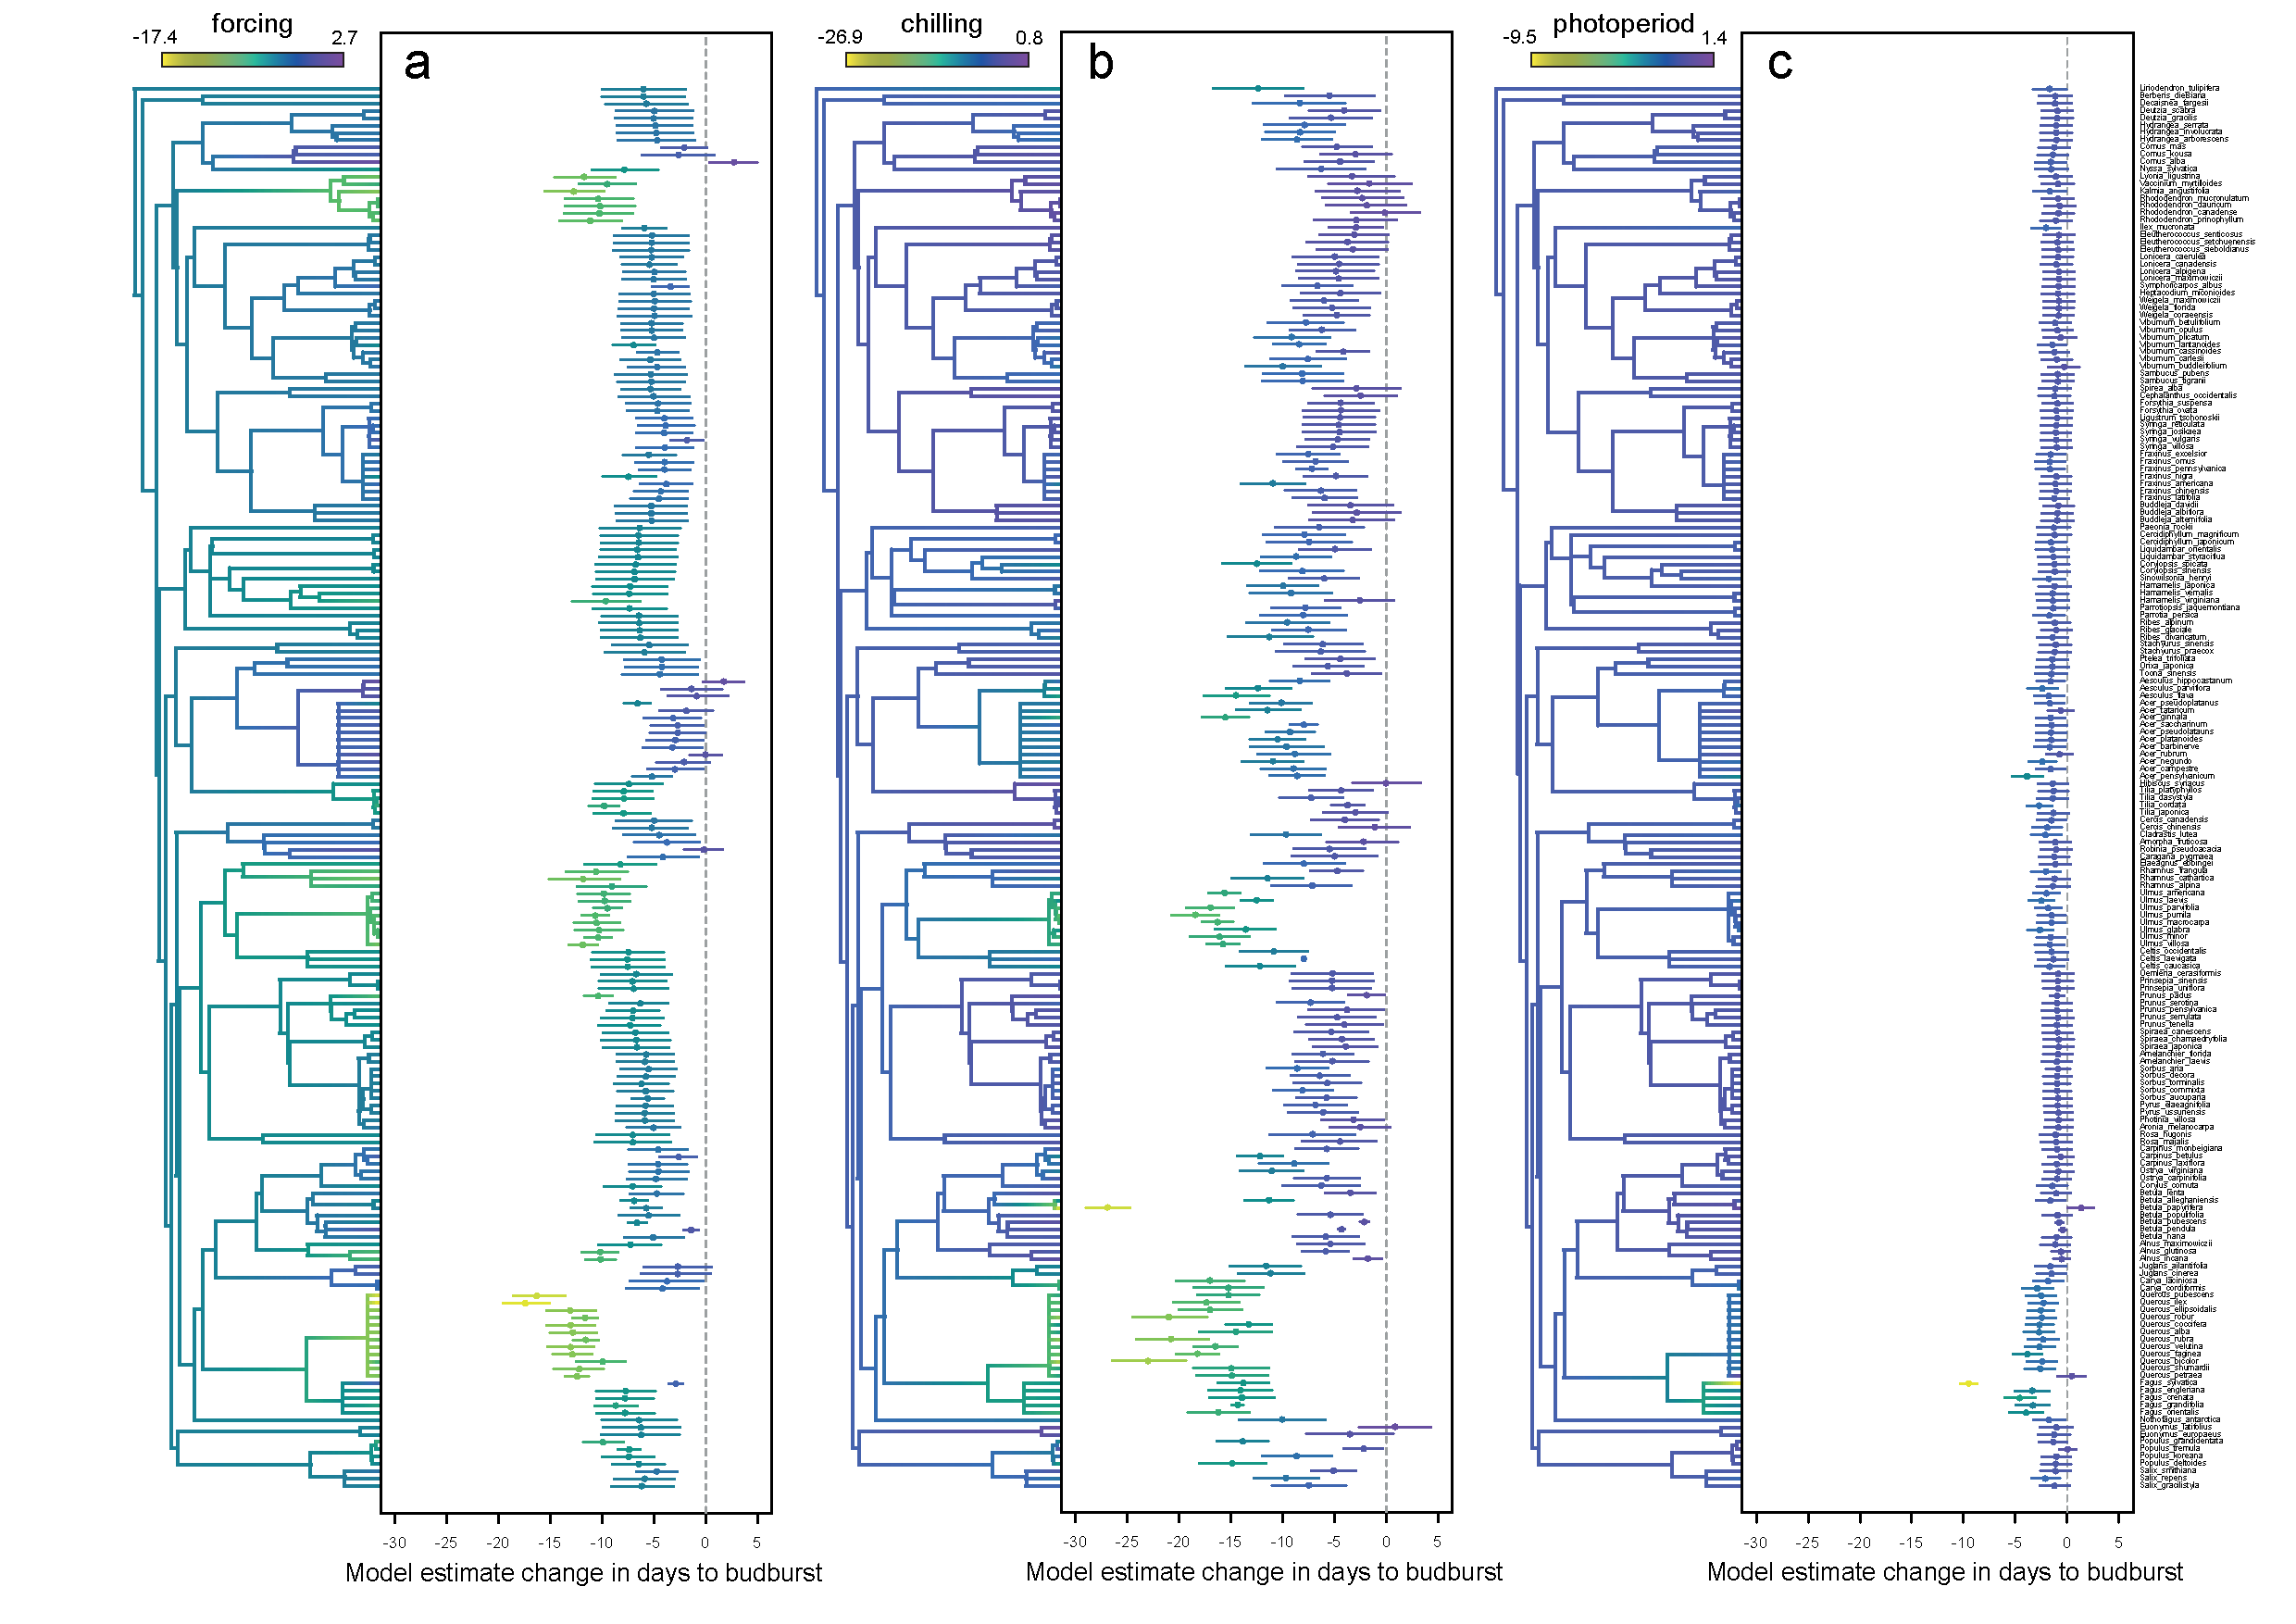
\includegraphics[width=16cm]{../../analyses/phylogeny/figures/muplot_phylo_allcue_angio.pdf}
  \caption{Phenological sensitivity to thee environmental cues, forcing (a), chilling (b) and photoperiod (c) measured in change in days to budburst per standardized unit (z-transformation) of the cues across 192 angiosperm species. The same phylogenetic tree is shown in each panel, colored acording to an estimation of ancestral character states, being the states at the tips the model slopes of our hierarchical phylogenetic model. Note that the color scale varies in each panel. Total tree depth is 81. My.}
  \label{fig:muplot_all}
  \end{center}
\end{figure}

\begin{figure} [H]
  \begin{center}
  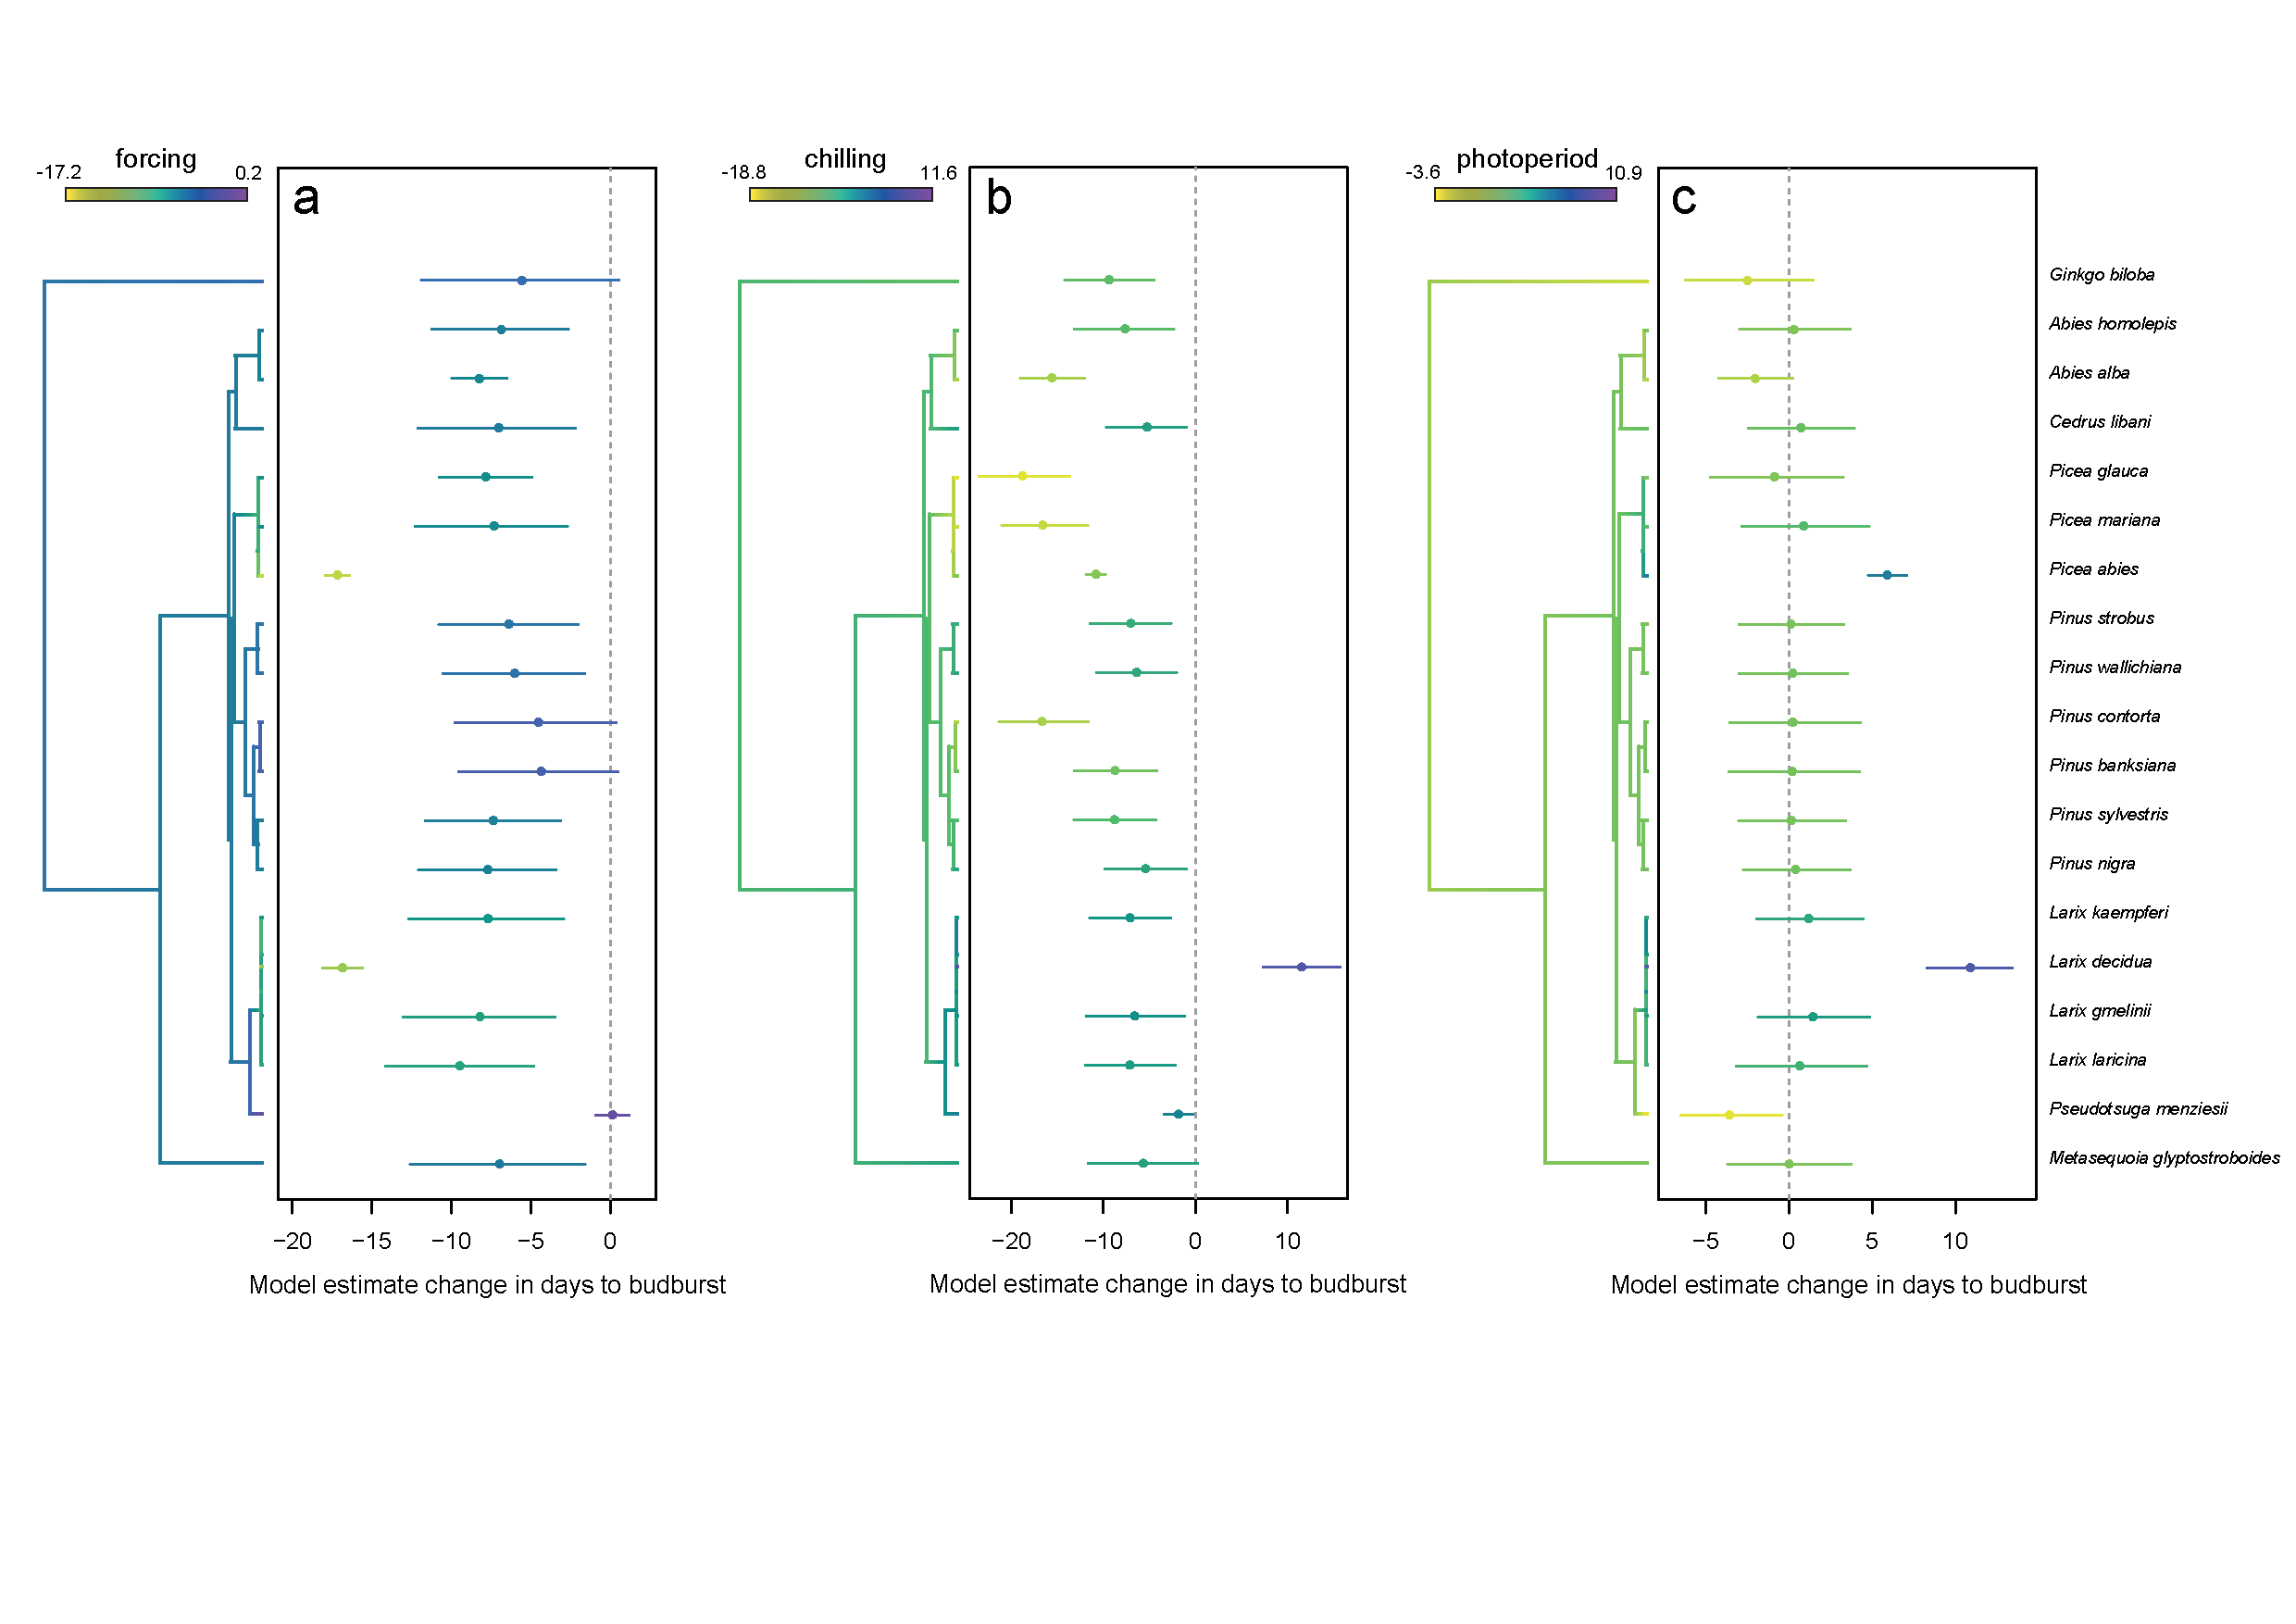
\includegraphics[width=16cm]{../../analyses/phylogeny/figures/Fig1b_phylo_muplots_gymno.pdf}
  \caption{Phenological sensitivity to thee environmental cues, forcing (a), chilling (b) and photoperiod (c) measured in change in days to budburst per standardized unit (z-transformation) of the cues across 19 gymnosperm species. The same phylogenetic tree is shown in each panel, colored acording to an estimation of ancestral character states, being the states at the tips the model slopes of our hierarchical phylogenetic model. Note that the color scale varies in each panel. Total tree depth is 81. My.}
  \label{fig:muplot_allgymno}
  \end{center}
\end{figure}


\begin{figure} [H]
  \begin{center}
  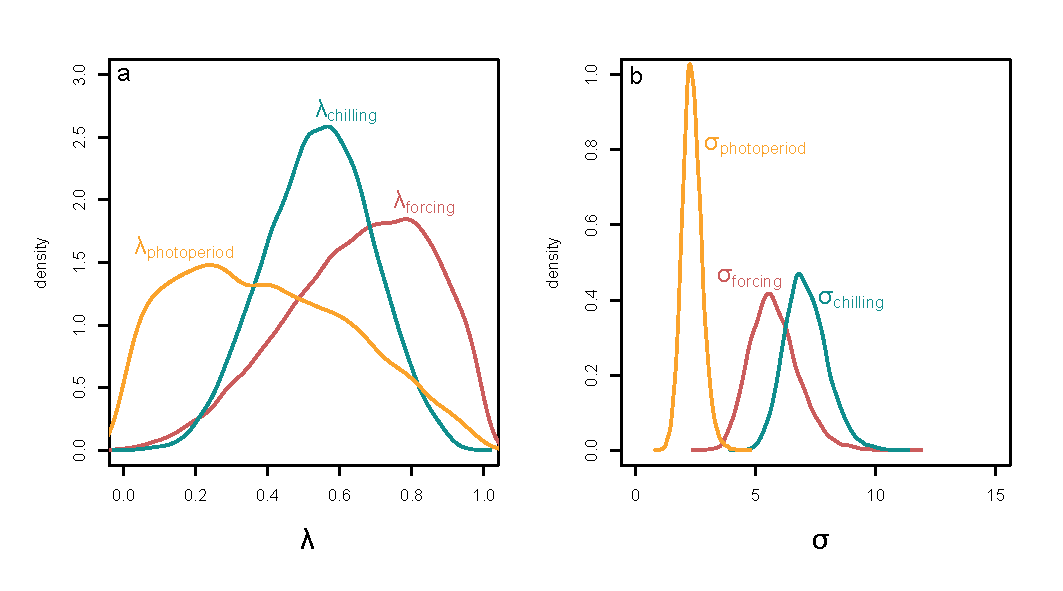
\includegraphics[width=14cm]{../../analyses/phylogeny/figures/Fig2_lambdas_sigmas.pdf}
  \caption{Density plots for the posterior distribution of phylogenetic signal measured by lambda for each cue included as a predictor in the model for angiosperms: forcing (red), chilling (blue),  photoperiod (orange) and for the model intercept (grey). Panels correspond to angiosperms (a-d) and gymnosperms (e-h). Note that lambda estimations corresponding to  panels c-d and g-h as they are constrained to be either equal zero or equal 1.}
  \label{fig:phylosig_all}
  \end{center}
\end{figure}

\begin{figure} [H]
  \begin{center}
  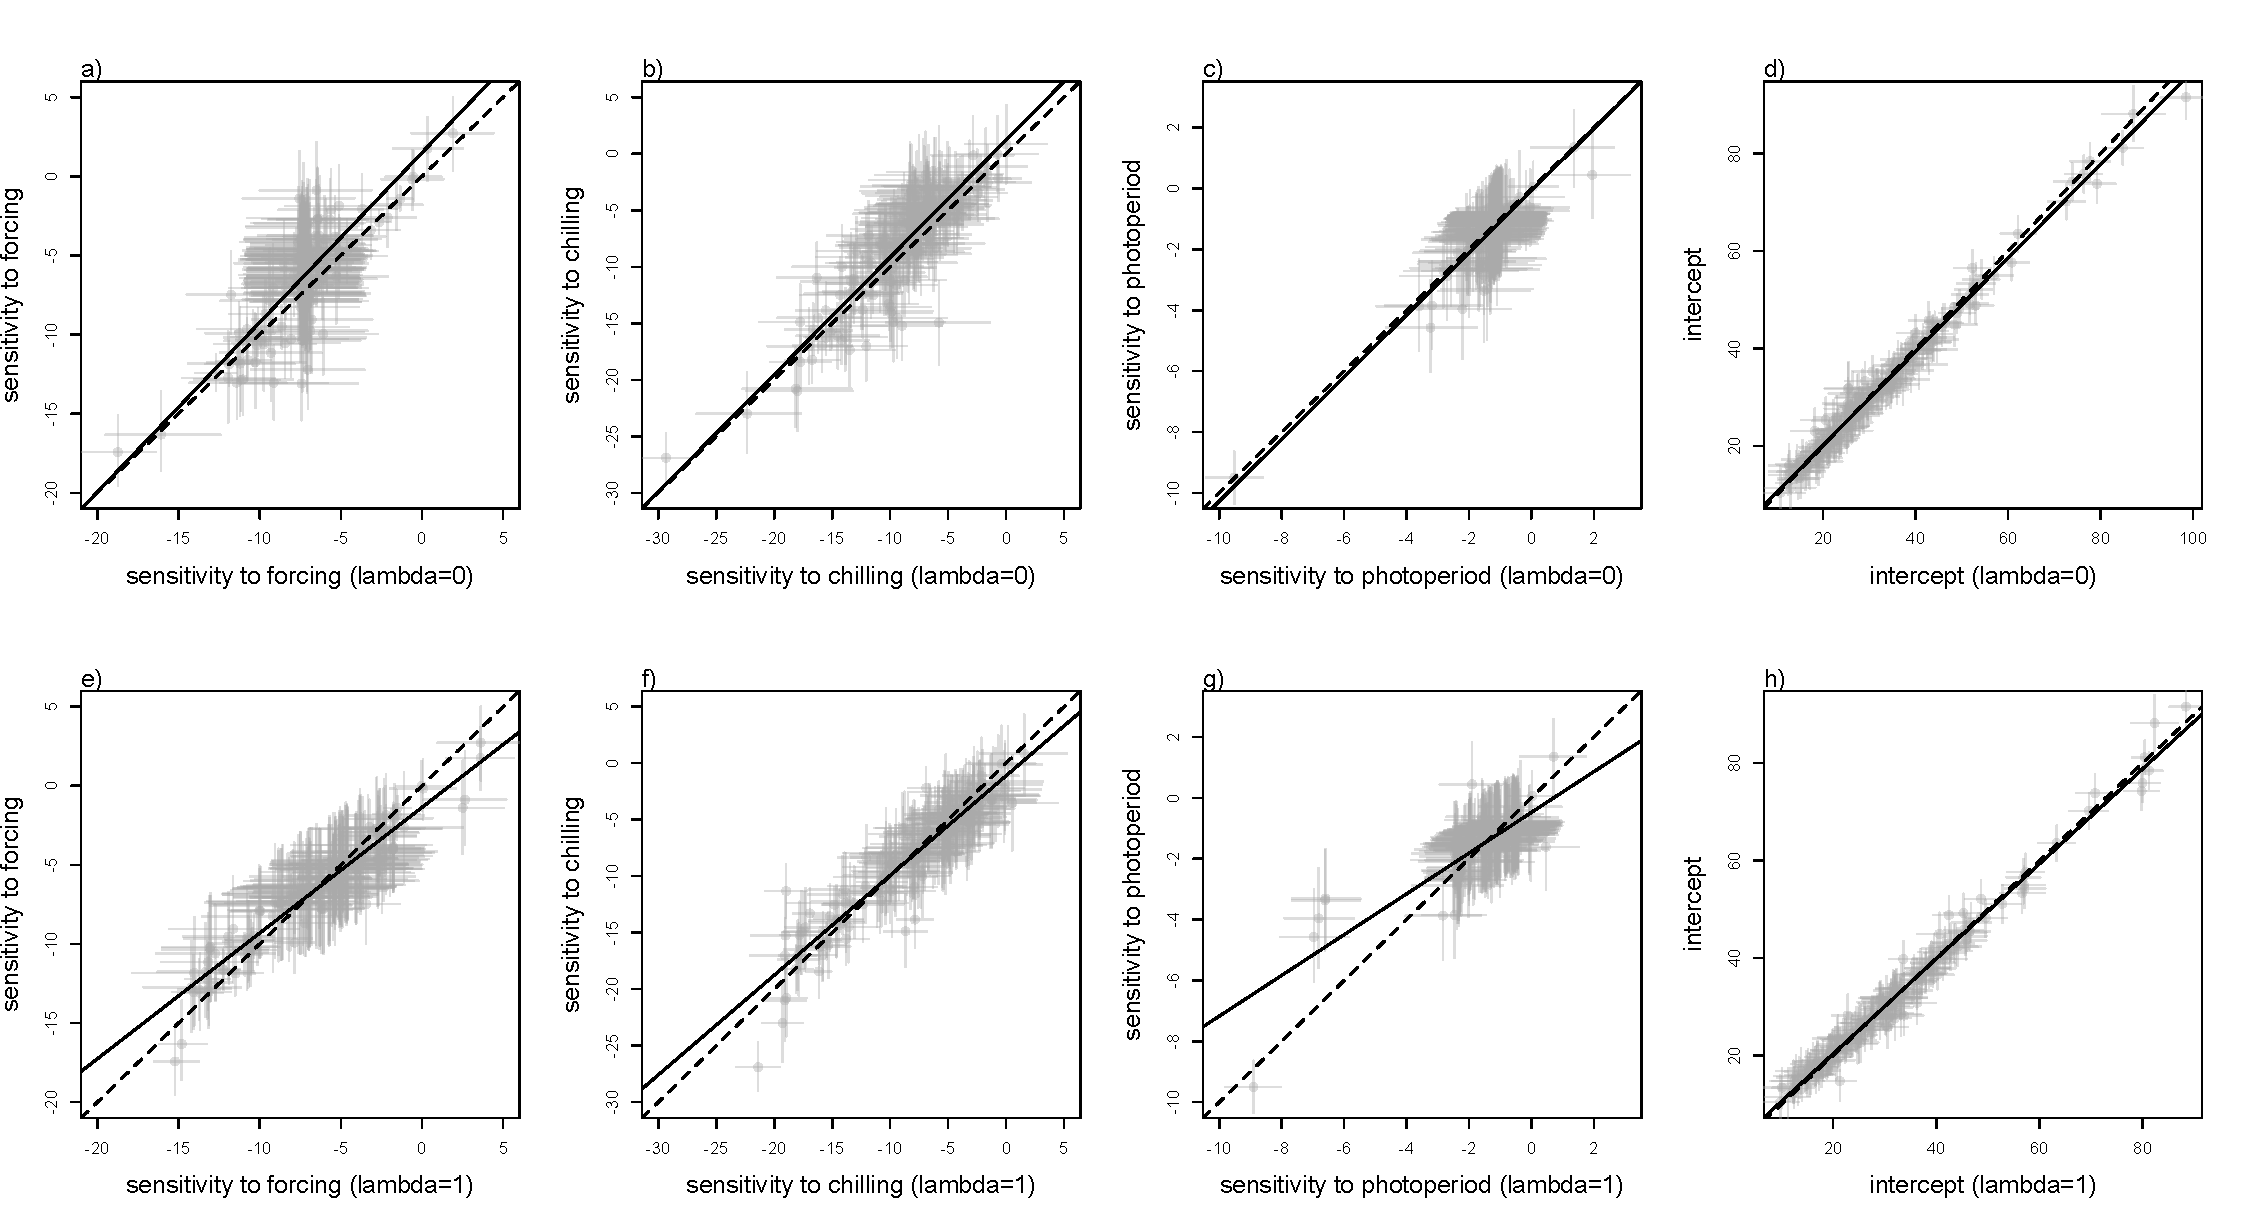
\includegraphics[width=14cm]{../../analyses/phylogeny/figures/Est_correls_vs_lamb01_angio.pdf}
  \caption{Correlations between model parameters as estimated by the full model and the models where lambda is constrained to be equal zero (upper row) or one (bottom row), for angiosperms. Panels correspond to sensitivity to forcing (a,e), to chilling (b,f), to photoperiod (c,g) and to model intercepts (d,h).}
  \label{fig:correls_angio}
  \end{center}
\end{figure}

\begin{figure} [H]
  \begin{center}
  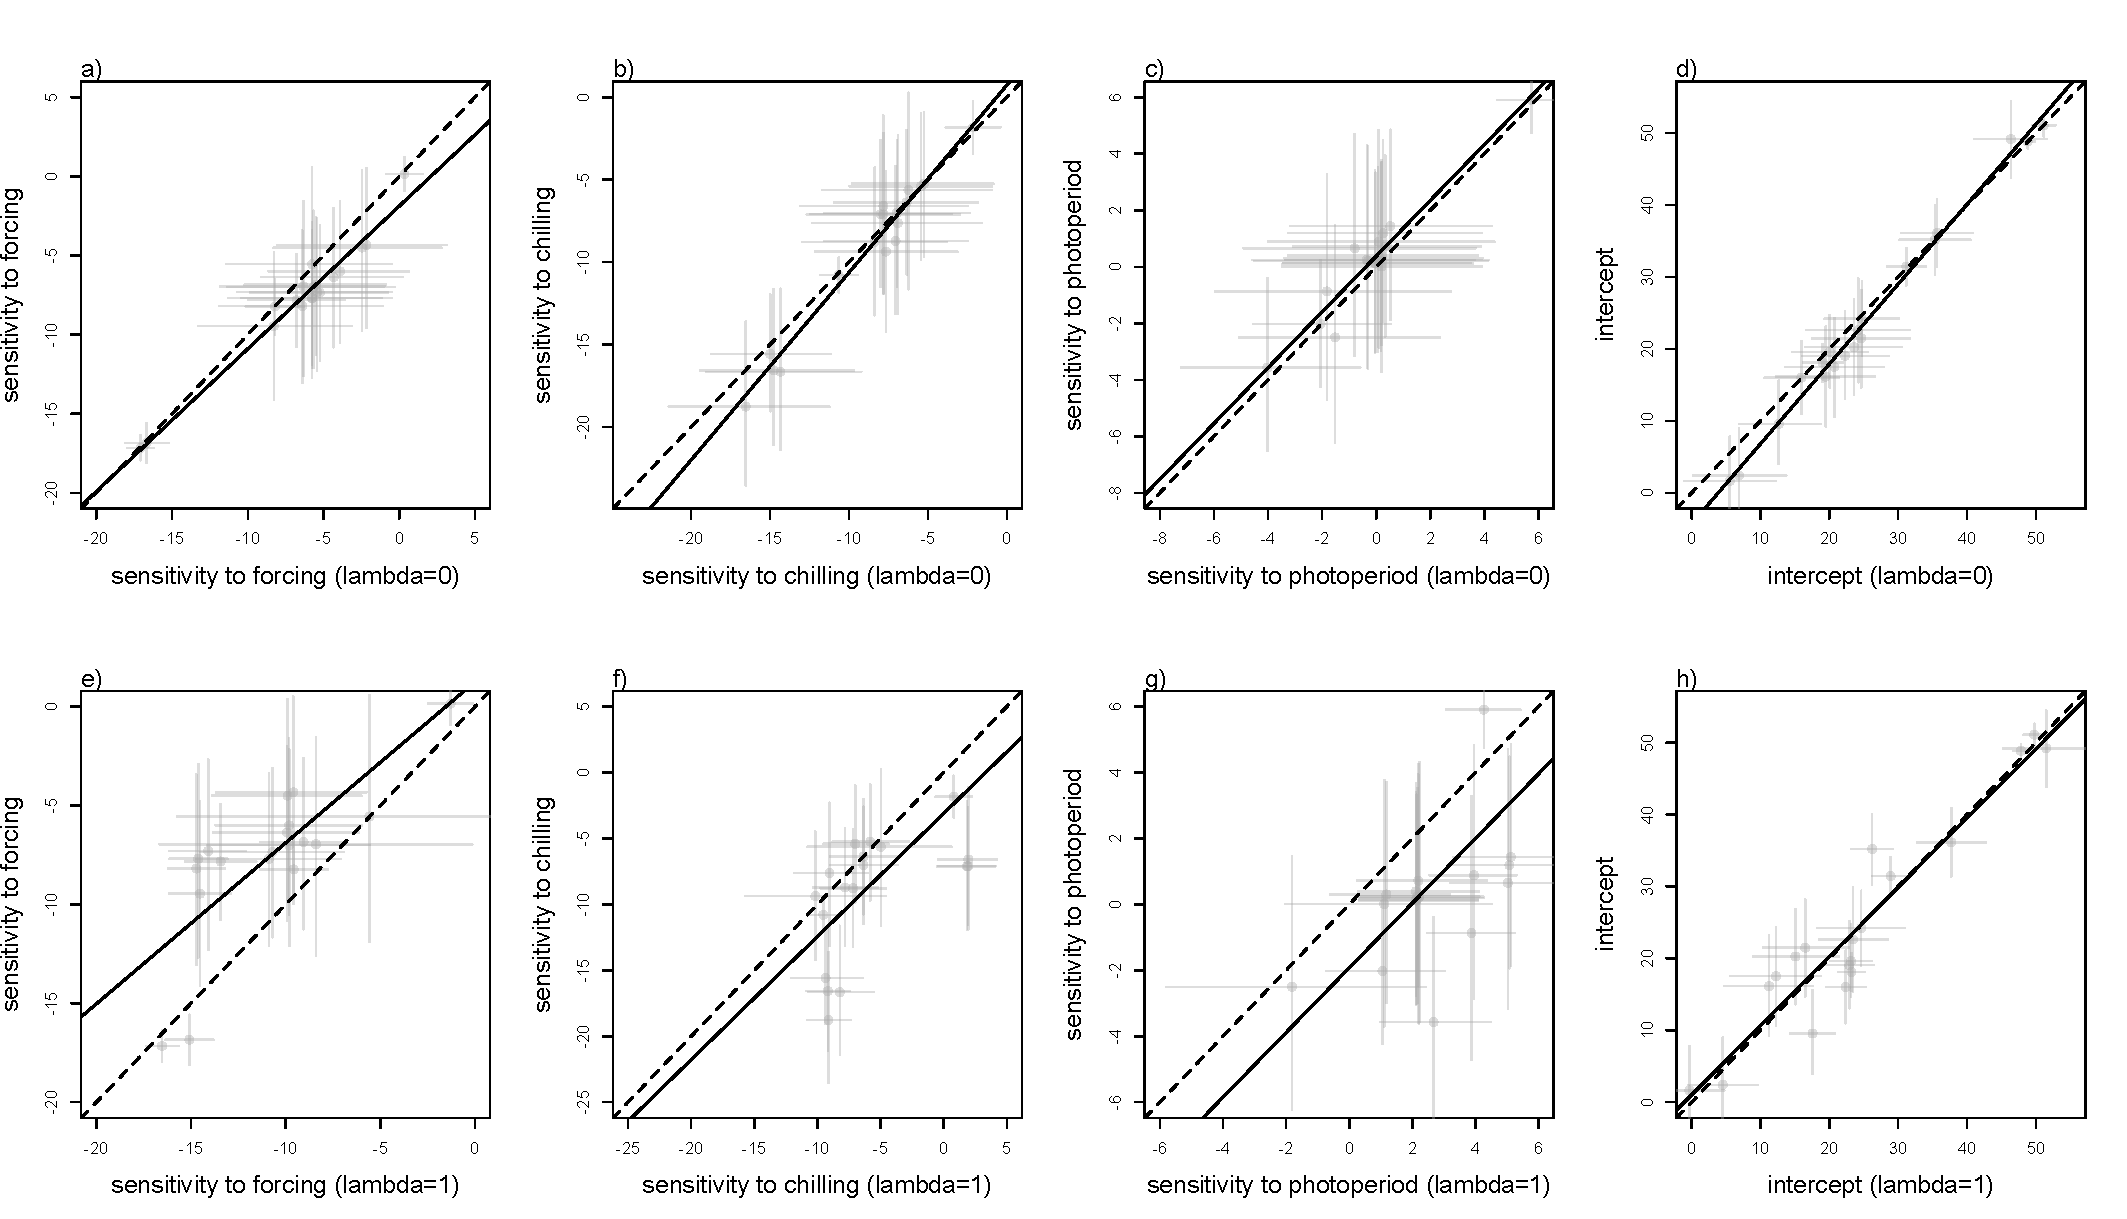
\includegraphics[width=14cm]{../../analyses/phylogeny/figures/Est_correls_vs_lamb01_gymno.pdf}
  \caption{Correlations between model parameters as estimated by the full model and the models where lambda is constrained to be equal zero (upper row) or one (bottom row), for gymnosperms. Panels correspond to sensitivity to forcing (a,e), to chilling (b,f), to photoperiod (c,g) and to model intercepts (d,h).}
  \label{fig:correls_gymno}
  \end{center}
\end{figure}



% IMC Mar21 - I'm guessing we are going to merge some of the tables below. TBD what we keep for the main text and what is sent to a supp.
\begin{table}[H]
\begin{center}
\caption{Full model parameters estimated for 192 angiosperm species.}
\begin{tabular}{@{}lcccccc@{}}
\toprule
\textbf{parameter}             & \multicolumn{1}{l}{\textbf{mean}} & \multicolumn{1}{l}{\textbf{sd}} & \multicolumn{1}{l}{\textbf{2.50\%}} & \multicolumn{1}{l}{\textbf{50\%}} & \multicolumn{1}{l}{\textbf{97.50\%}} & \multicolumn{1}{l}{\textbf{n\_eff}} \\ \midrule
$\mu_\alpha$                   & 30.57                             & 3.41                            & 23.68                               & 30.59                             & 37.14                                & 5031.19                             \\
$\mu_\beta_{forcing}$          & -5.84                             & 2.01                            & -9.72                               & -5.89                             & -1.79                                & 2374.73                             \\
$\mu_\beta_{chilling}$         & -7.19                             & 2.03                            & -11.15                              & -7.18                             & -3.18                                & 3694.93                             \\
$\mu_\beta_{photoperiod}$      & -1.37                             & 0.76                            & -2.92                               & -1.35                             & 0.14                                 & 1565.41                             \\
$\lambda_\alpha$               & 0.35                              & 0.10                            & 0.16                                & 0.34                              & 0.56                                 & 3416.51                             \\
$\lambda_\beta_{forcing}$      & 0.68                              & 0.20                            & 0.23                                & 0.71                              & 0.98                                 & 185.35                              \\
$\lambda_\beta_{chilling}$     & 0.56                              & 0.15                            & 0.25                                & 0.56                              & 0.83                                 & 738.57                              \\
$\lambda_\beta_{photoperiod}$  & 0.36                              & 0.24                            & 0.02                                & 0.33                              & 0.88                                 & 296.51                              \\
$\sigma_\alpha^2$              & 15.93                             & 1.17                            & 13.84                               & 15.85                             & 18.41                                & 2988.37                             \\
$\sigma_\beta^2_{forcing}$     & 5.84                              & 1.04                            & 4.03                                & 5.78                              & 8.15                                 & 502.74                              \\
$\sigma_\beta^2_{chilling}$    & 7.05                              & 0.87                            & 5.48                                & 7.02                              & 8.92                                 & 1026.77                             \\
$\sigma_\beta^2_{photoperiod}$ & 2.45                              & 0.41                            & 1.74                                & 2.42                              & 3.32                                 & 469.46                              \\
$\sigma_y^2$                   & 12.81                             & 0.18                            & 12.47                               & 12.80                             & 13.17                                & 4017.16                             \\ \bottomrule
\end{tabular}
\end{center}
\label{tab:modelanglamb}
\end{table}


\begin{table}[H]
 \begin{center}
\caption{Full model parameters estimated for 19 gymnosperm species.}
\begin{tabular}{@{}lcccccc@{}}
\toprule
\textbf{parameter}             & \multicolumn{1}{l}{\textbf{mean}} & \multicolumn{1}{l}{\textbf{sd}} & \multicolumn{1}{l}{\textbf{2.50\%}} & \multicolumn{1}{l}{\textbf{50\%}} & \multicolumn{1}{l}{\textbf{97.50\%}} & \multicolumn{1}{l}{\textbf{n\_eff}} \\ \midrule
$\mu_\alpha$                   & 25.75                             & 4.50                            & 16.88                               & 25.73                             & 34.73                                & 33151.86                            \\
$\mu_\beta_{forcing}$          & -5.92                             & 3.80                            & -12.97                              & -6.05                             & 1.90                                 & 16443.03                            \\
$\mu_\beta_{chilling}$         & -8.11                             & 3.63                            & -15.31                              & -8.09                             & -0.94                                & 21379.81                            \\
$\mu_\beta_{photoperiod}$      & -0.88                             & 3.33                            & -8.01                               & -0.67                             & 5.19                                 & 16301.93                            \\
$\lambda_\alpha$               & 0.47                              & 0.26                            & 0.02                                & 0.48                              & 0.90                                 & 15934.03                            \\
$\lambda_\beta_{forcing}$      & 0.36                              & 0.23                            & 0.02                                & 0.33                              & 0.84                                 & 14336.60                            \\
$\lambda_\beta_{chilling}$     & 0.32                              & 0.23                            & 0.01                                & 0.28                              & 0.82                                 & 13230.88                            \\
$\lambda_\beta_{photoperiod}$  & 0.37                              & 0.24                            & 0.02                                & 0.34                              & 0.88                                 & 11199.49                            \\
$\sigma_\alpha^2$              & 23.47                             & 6.20                            & 13.87                               & 22.59                             & 37.81                                & 18272.58                            \\
$\sigma_\beta^2_{forcing}$     & 8.89                              & 2.45                            & 4.96                                & 8.60                              & 14.51                                & 8126.51                             \\
$\sigma_\beta^2_{chilling}$    & 10.47                             & 2.66                            & 5.78                                & 10.30                             & 16.17                                & 8539.38                             \\
$\sigma_\beta^2_{photoperiod}$ & 7.18                              & 2.29                            & 3.29                                & 6.96                              & 12.25                                & 5625.69                             \\
$\sigma_y^2$                   & 15.81                             & 0.41                            & 15.04                               & 15.81                             & 16.63                                & 28640.16                            \\ \bottomrule
\end{tabular}
\end{center}
\label{tab:modelgymlamb}
\end{table}





\pagebreak
%\bibliographystyle{refs/bibstyles/amnat.bst}% 
%\bibliography{refs/phylorefs.bib}



\end{document}
